\documentclass[a4paper, 11pt]{article}
\usepackage[utf8]{inputenc}
\usepackage{float}
\usepackage{graphicx}
\usepackage{url}
\usepackage{enumitem}
\usepackage{subcaption}

\setlist[itemize]{itemsep=0.5pt, parsep=0.5pt, topsep=0pt, partopsep=0pt}
\setlist[enumerate]{itemsep=0.5pt, parsep=0.5pt, topsep=0pt, partopsep=0pt}

%opening
\title{HW3 Report, Loggy: A Logical Time Logger}
\author{David Fischer}
\date{\today{}}

\begin{document}

\maketitle

\section{Introduction}
Lamport and vector clocks serve as fundamental tools that enable causal ordering in distributed systems. Though implementations might differ, their core principles are still represented in multiple areas such as distributed tracing, message queues, and distributed garbage collection.
This assignments goal was the implementation of \textit{Loggy}, a logging procedure continually receiving random messages on a random delay from workers.

The implementation spans a central logging module with a holdback queue to correctly print messages, workers sending and receiving messages between each other on a random delay with random jitters before reporting to the central logger, two clock modules, Lamport and vector based, and multiple analytics modules to generate insights.

\section{Main problems and solutions}

\subsection{Validating Order}



% something about difficulties validating if the clocks, especially the vector clocks, are functioning correctly, solved in chart maker with evaluation

\subsection{Log Parsing}

% difficulty reading the log until the log output was made clean using the built in padding

\subsection{Holdback Queue Implementation}

% from assignment: How do we know if messages are safe to print?
% from assignment: You are also to write a report that describes your time module
% holdback queue implementation, difficulty mentally parsing the queue size/why it jumps so massively

% Did you detect entries out of order in the first implementation, and if so, how did you detect them? 
% What is it that the final log tells us? Did events happen in the order presented by the log? 
% How large will the holdback queue be, make some tests and try to find the maximum number of entries.

%Did events happen in the order presented by the log?
%How large will the holdback queue be, make some tests and try to find the maximum number of entries.

\section{Evaluation}

% Do some tests and identify situations where log entries are printed in the wrong order. 
% How do you identify messages that are in the wrong order?
% What is always true, and what is sometimes true? How do you play it safe?

\subsection{Visualization}

To aid evaluation, a module \textit{mermaid} was implemented to create visual representations of the messages flowing between the vector clocks.

See appendix. (TODO, proper sendoff to the appendix, google how)

\subsection{Queue Size Comparison}


\begin{figure}[H]
  \begin{center}
    \begin{subfigure}[b]{0.494\textwidth}
      \centering
      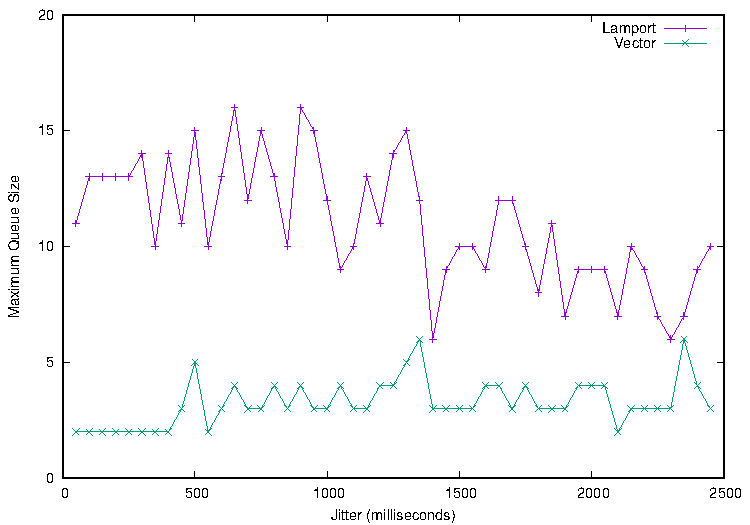
\includegraphics[width=\textwidth]{test/jitter.pdf}
      \caption{Comparison of Jitter using a 1500ms Sleep}
      \label{fig:results1}
    \end{subfigure}
    \hfill
    \begin{subfigure}[b]{0.494\textwidth}
      \centering
      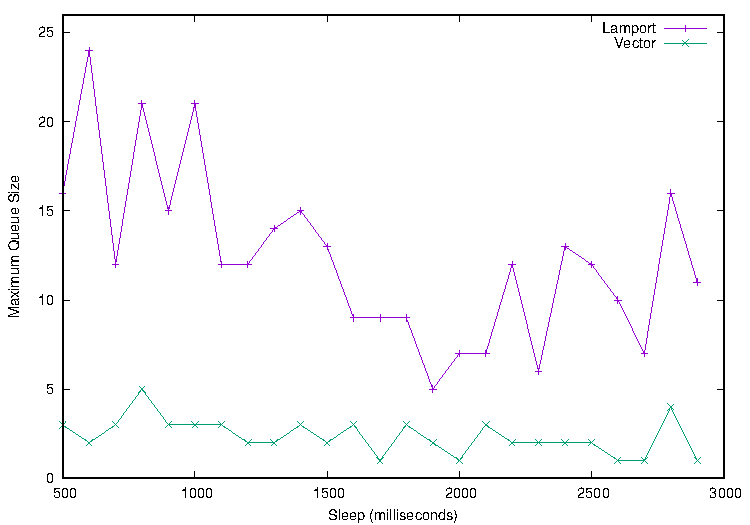
\includegraphics[width=\textwidth]{test/sleep.pdf}
      \caption{Comparison of Sleep using a 250ms Jitter}
      \label{fig:results2}
    \end{subfigure}
  \end{center}
  \caption{Queue size comparison between the clock implementations on different delays and jitters}
  \label{fig:comparison}
\end{figure}

Due to the inherit randomness of the \textit{Loggy} implementation these results can't be taken as absolutes for corelating sleep or jitter to the maximum queue size.
Still, the difference between the maximum size of the Lamport queue when compared to the vector queue demonstrates the logging throughput being greater, at the cost of larger messages.

% actually validate that the queue size isn't too big, logging seems weird right now, 
% CONFIRMED: i'm just stupid the queue size is always printed by all the same logging outs


\section{Conclusions}

% Is this not exactly what we have done in the Lamport clock solution?

An interesting part of this \textit{Loggy} implementation was the similarity between the full Lamport clock and the individual times held by the vector clock workers.
Concluding, the vector implementation is similar to the Lamport implementation at its core due to the shared methodology of incrementing a simple value to represent [the state in time ]


% something about vector clocks


\newpage
\section{Appendix}

Both of these tests were completed using test:run(<module>, 1500, 500).

\subsection{Lamport Clock}
\begin{verbatim}
119> test:run(time, 1500, 500).
loggy: starting with module time
log: s:5   ringo  sending  ( 24) c:1
log: s:5   john   sending  (  6) c:1
log: s:5   george sending  ( 26) c:1
log: s:2   paul   received ( 24) c:2
log: s:2   john   received ( 26) c:2
log: s:2   paul   received (  6) c:3
log: s:2   john   sending  ( 50) c:3
log: s:2   ringo  received ( 50) c:4
log: s:2   john   sending  ( 73) c:4
log: s:2   paul   sending  ( 28) c:4
log: s:8   george received ( 28) c:5
log: s:8   ringo  sending  (  2) c:5
log: s:8   john   sending  ( 37) c:5
log: s:13  george received ( 73) c:6
log: s:13  paul   received (  2) c:6
log: s:13  john   sending  (  1) c:6
log: s:3   george sending  ( 48) c:7
log: s:3   paul   sending  ( 30) c:7
log: s:3   ringo  received ( 48) c:8
log: s:3   paul   received ( 37) c:8
log: s:3   ringo  sending  ( 86) c:9
log: s:3   george received ( 86) c:10
log: s:3   george received ( 30) c:11
log: s:3   george sending  ( 85) c:12
log: s:3   ringo  received ( 85) c:13
log: s:3   ringo  sending  ( 83) c:14
log: s:3   george received ( 83) c:15
log: s:3   ringo  received (  1) c:15
\end{verbatim}
% \caption{Test execution of the lamport clock}

\begin{figure}[H]
  \begin{center}
    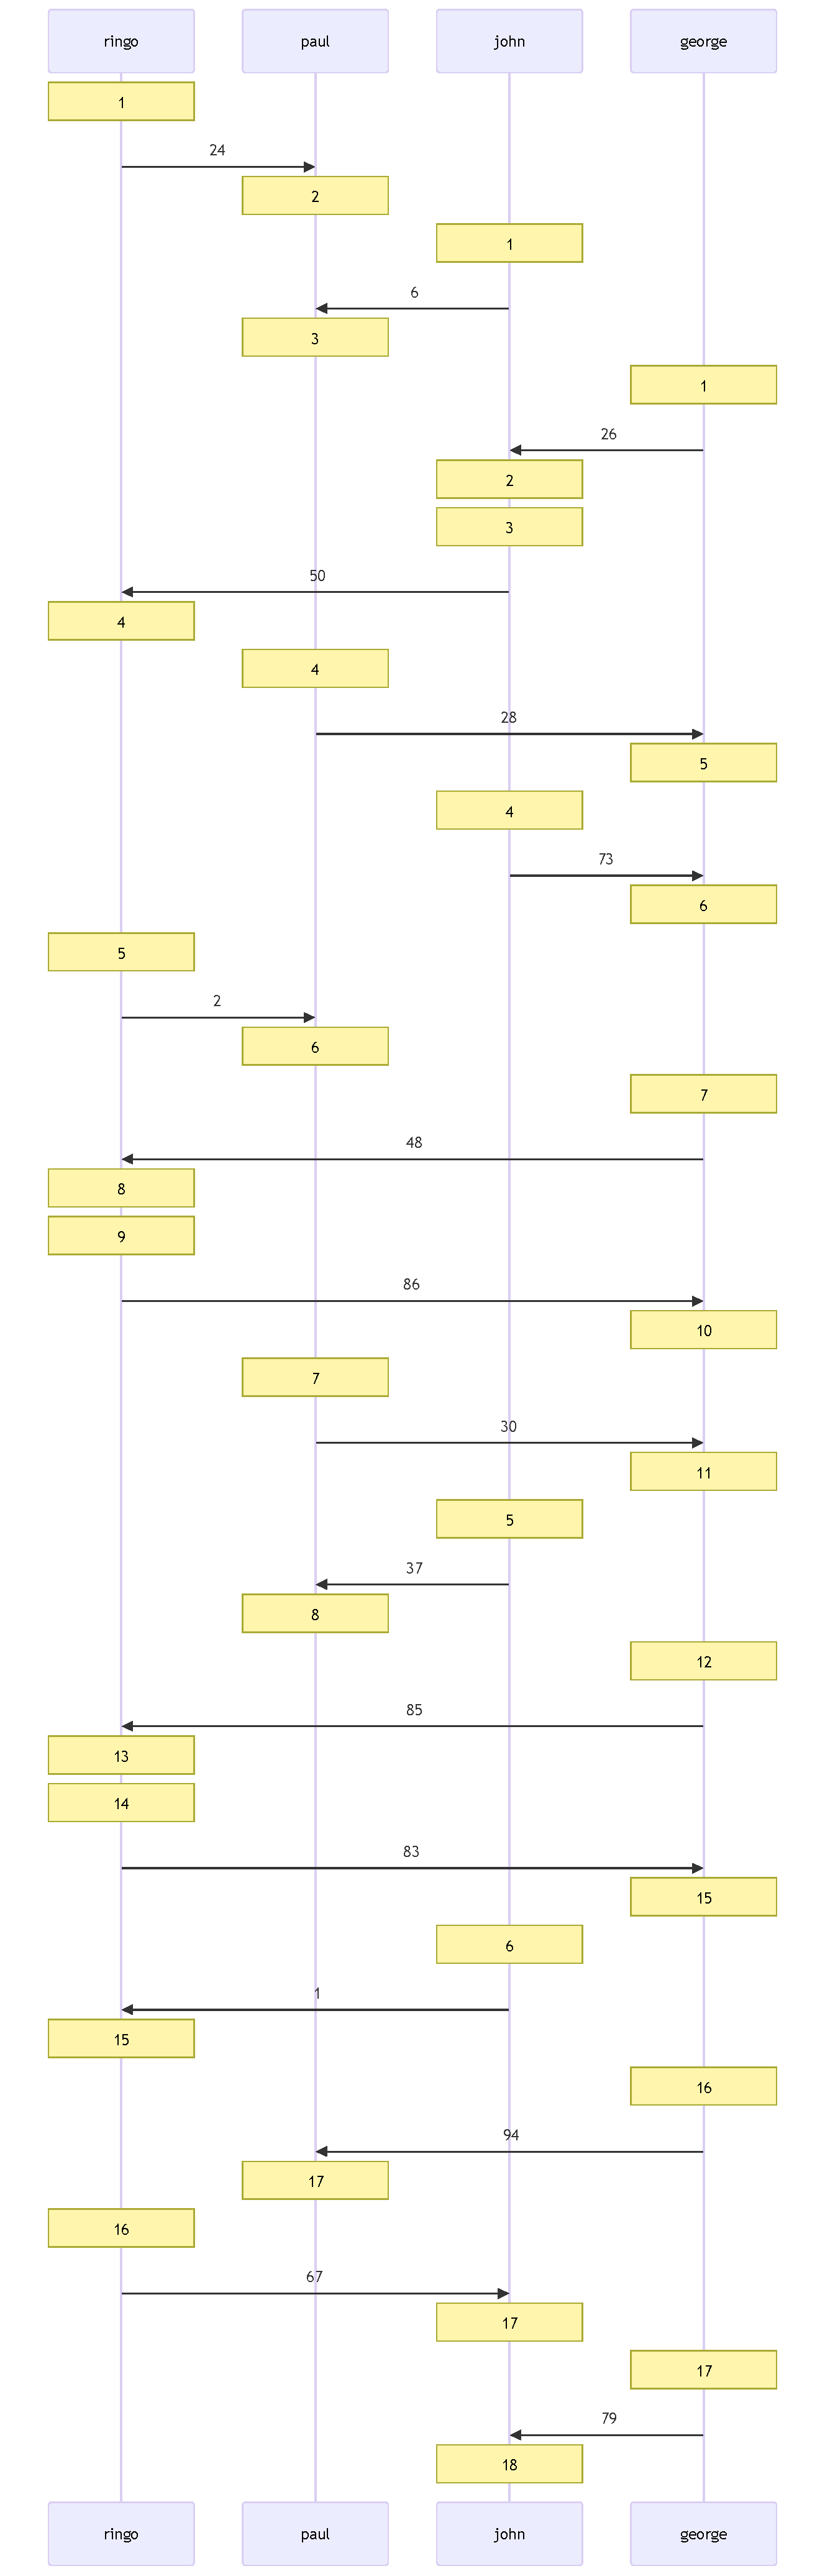
\includegraphics[height=\textheight]{graphics/mermaid_lamport.pdf}
    \caption{Sequence visualization of the Lamport timestamp algorithm}
    \label{fig:seq1}
  \end{center}
\end{figure}

\subsection{Vector Clock}
\begin{verbatim}
120> test:run(vect, 1500, 500).
loggy: starting with module vect
log: s:1   ringo  sending  ( 24) c:ringo => 1
log: s:1   paul   received ( 24) c:paul => 1,ringo => 1
log: s:0   john   sending  (  6) c:john => 1
log: s:0   paul   received (  6) c:john => 1,paul => 2,ringo => 1
log: s:0   george sending  ( 26) c:george => 1
log: s:0   john   received ( 26) c:john => 2,george => 1
log: s:0   john   sending  ( 50) c:john => 3,george => 1
log: s:0   ringo  received ( 50) c:john => 3,ringo => 2,george => 1
log: s:2   john   sending  ( 73) c:john => 4,george => 1
log: s:0   paul   sending  ( 28) c:john => 1,paul => 3,ringo => 1
log: s:0   george received ( 28) c:john => 1,paul => 3,ringo => 1,george => 2
log: s:0   george received ( 73) c:john => 4,paul => 3,ringo => 1,george => 3
log: s:0   ringo  sending  (  2) c:john => 3,ringo => 3,george => 1
log: s:0   paul   received (  2) c:john => 3,paul => 4,ringo => 3,george => 1
log: s:0   george sending  ( 48) c:john => 4,paul => 3,ringo => 1,george => 4
log: s:0   ringo  received ( 48) c:john => 4,paul => 3,ringo => 4,george => 4
log: s:1   john   sending  ( 37) c:john => 5,george => 1
log: s:1   paul   received ( 37) c:john => 5,paul => 5,ringo => 3,george => 1
log: s:0   ringo  sending  ( 86) c:john => 4,paul => 3,ringo => 5,george => 4
log: s:0   george received ( 86) c:john => 4,paul => 3,ringo => 5,george => 5
log: s:2   george sending  (  8) c:john => 4,paul => 3,ringo => 5,george => 6
log: s:1   ringo  sending  ( 84) c:john => 4,paul => 3,ringo => 6,george => 4
log: s:1   paul   received ( 84) c:john => 5,paul => 6,ringo => 6,george => 4
log: s:1   paul   received (  8) c:john => 5,paul => 7,ringo => 6,george => 6
log: s:1   paul   sending  ( 46) c:john => 5,paul => 8,ringo => 6,george => 6
log: s:1   george received ( 46) c:john => 5,paul => 8,ringo => 6,george => 7
log: s:1   john   sending  (  1) c:john => 6,george => 1
log: s:1   ringo  received (  1) c:john => 6,paul => 3,ringo => 7,george => 4
log: s:0   george sending  ( 99) c:john => 5,paul => 8,ringo => 6,george => 8
log: s:0   paul   received ( 99) c:john => 5,paul => 9,ringo => 6,george => 8
\end{verbatim}

\begin{figure}[H]
  \begin{center}
    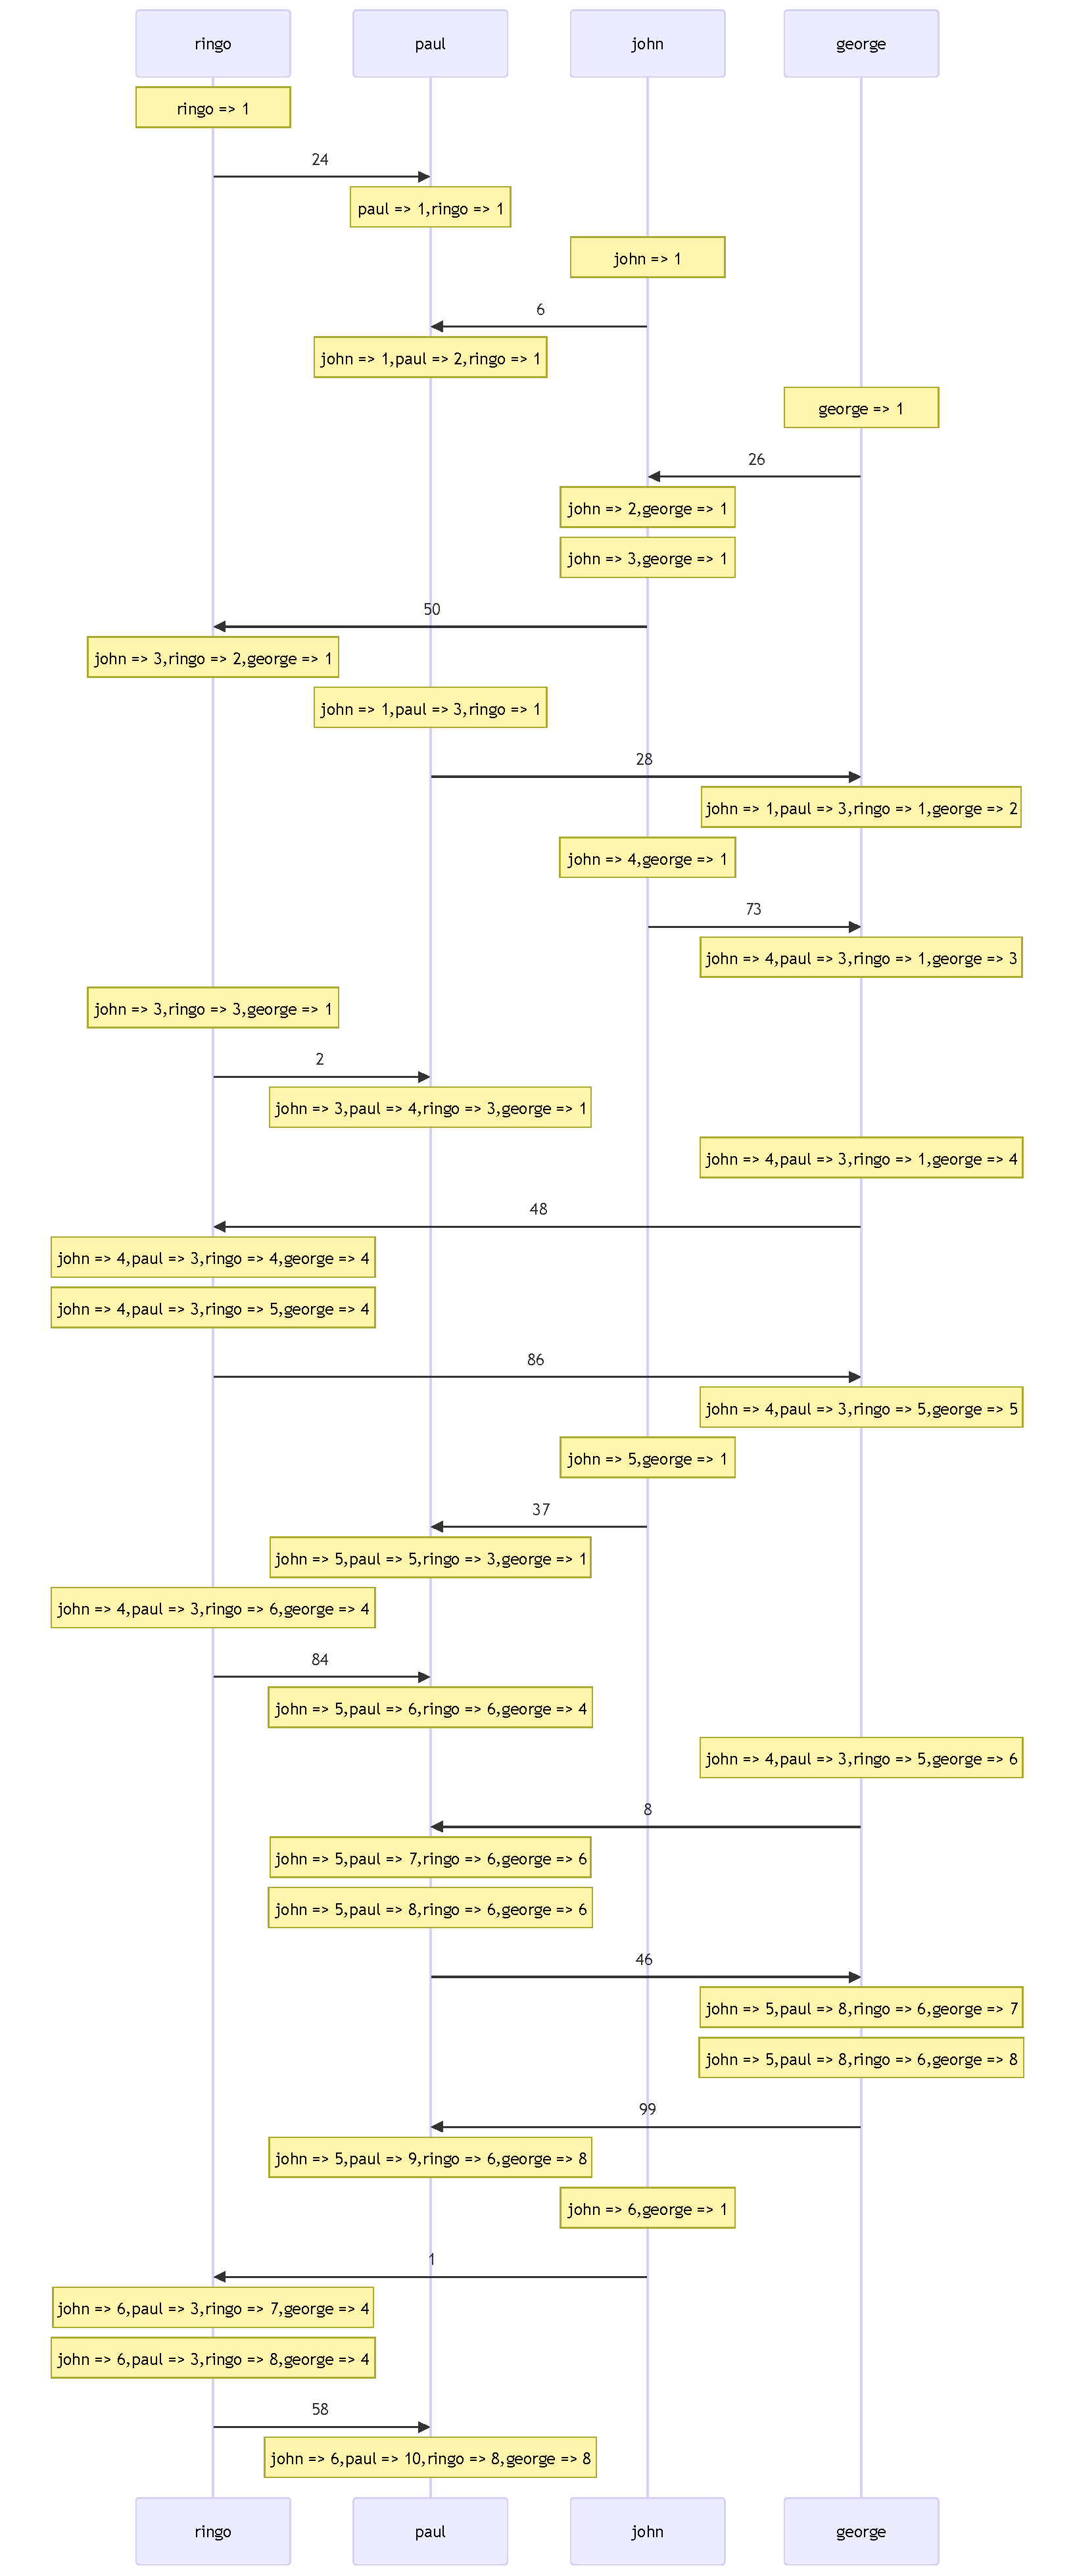
\includegraphics[height=\textheight]{graphics/mermaid_vector.pdf}
    \caption{Sequence visualization of the vector clock implementation}
    \label{fig:seq2}
  \end{center}
\end{figure}

\end{document}
